%! Author = Dean Didion
%! Date = 09.07.25

\chapter{Introduction}\label{ch:introduction}


\section{Motivation and relevance}\label{sec:motivation}

Innovation in the public sector is increasingly seen as essential for tackling complex societal challenges.
As governments and public institutions explore new ways to deliver services, assess policy outcomes, and engage with citizens, the question of \textbf{impact} becomes central.
While private sector innovations often measure success through profit and efficiency, public sector innovation needs to be evaluated against broader societal value, which is a much more nuanced and multidimensional goal.

Artificial Intelligence (AI) has emerged as a powerful tool for analyzing vast datasets, identifying complex patterns, and supporting evidence-based decision-making~\parencite{russell2016artificial, marr2018data}.
In the public sector, AI holds significant promise for enhancing transparency, accountability, and responsiveness.
A recent study (see~\cite{cornell2024}) carried out on UK public service professionals showed that about 22\% actively use generative AI and 45\% are aware of AI tools in their area, it is still \textit{not routinely applied} to assess the impact of innovation initiatives.


\begin{figure}[H]
  \centering
  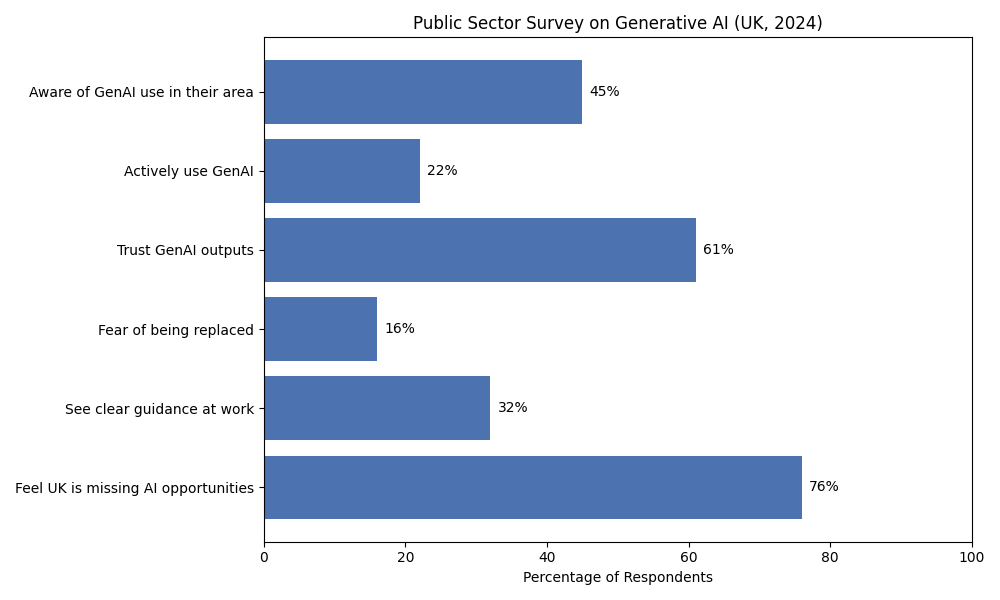
\includegraphics[width=0.8\textwidth]{../fig/ai_awareness_uk}
  \caption{Public sector professionals' attitudes toward generative AI ~\parencite{cornell2024}}
  \label{fig:genai_survey}
\end{figure}


Traditional impact measurement frameworks—while widely used—are often too rigid for the dynamic and experimental nature of many public sector initiatives (see Figure~\ref{fig:rigid_frameworks})
These frameworks may not accommodate evolving goals, emergent outcomes, or context-specific indicators.
Moreover, despite the variety of available frameworks, organizations tend to rely on a single predefined model, often because it is mandated or institutionally recognized.
This one-size-fits-all approach can limit flexibility and hinder meaningful evaluation.
There is, therefore, a growing need for more adaptive, intelligent systems that can integrate multiple perspectives and evolve alongside the initiatives they aim to assess.

\begin{figure}[H]
  \centering
  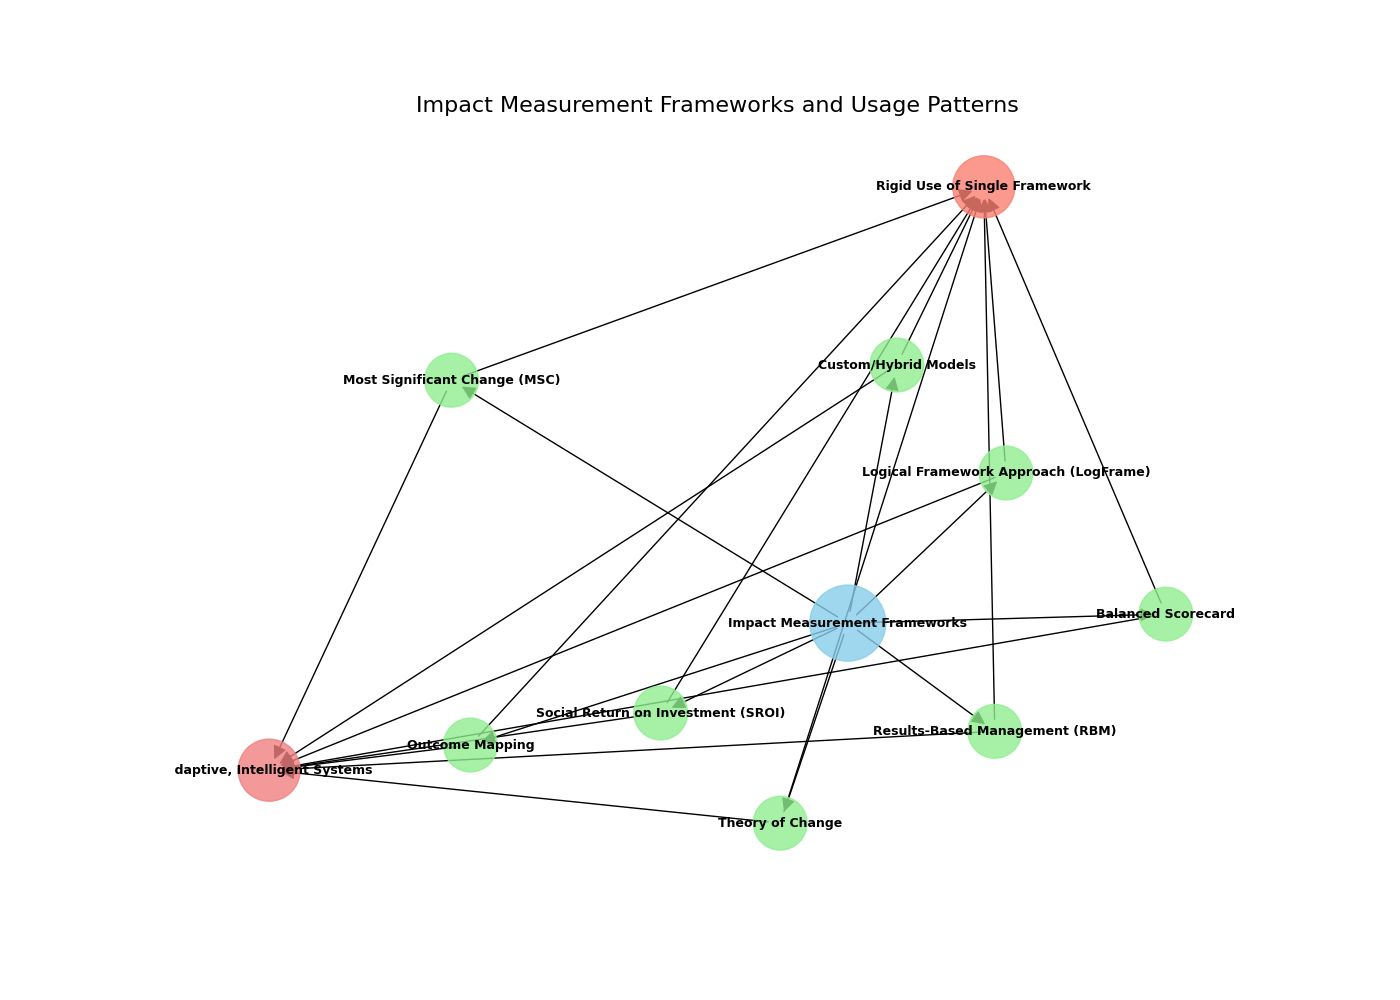
\includegraphics[width=0.8\textwidth]{../fig/rigid_use_frameworks}
  \caption{Rigid use of single frameworks}
  \label{fig:rigid_frameworks}
\end{figure}

This thesis is embedded in a real-world initiative from the \textbf{Public Value Hub in Leipzig} and aligns with the goals of the \textbf{Public Value Academy}, an emerging digital platform aimed at fostering innovation literacy and sustainable impact measurement in the public sector.

\section{Problem statement and research gap}\label{sec:problem-statement}
Despite the growing use of AI across sectors, there remains a significant gap in how AI can support \textbf{meaningful, qualitative impact assessment} — particularly in the public domain.
Existing tools often rely on rigid indicators and retrospective analysis, failing to capture complexity, learning, or long-term public value creation~\parencite{ebrahim2014impact, patton2011developmental}.
Moreover, public sector organizations often lack the resources or knowledge to adopt AI tools effectively~\parencite{mikhaylov2018ai}.
Furthermore, public sector organizations often do not have access to the resources or knowledge to adopt and adapt AI tools effectively.

There is a need to explore \textbf{how AI technologies can be applied to support dynamic, context-sensitive, and participatory impact measurement}, integrating frameworks such as those developed by \textbf{PHINEO} and supported by \textbf{UnternehmerTUM’s educational content}.

\section{Objectives}\label{sec:objectives}
The aim of this thesis is to develop a \textbf{conceptual and technical framework} for AI-supported impact measurement.
By combining theory, stakeholder insights, and prototyping with Python-based methods, the goal is to investigate how such a system could function in practice as part of the Public Value Academy’s software platform.

\section{Research questions}\label{sec:research-questions}

This thesis investigates the potential of artificial intelligence to enhance impact measurement practices.
Given the complexity and evolving nature of public value creation, the research is guided by the following questions:

\begin{itemize}
  \item \textbf{How can artificial intelligence contribute to improved impact measurement in public sector innovation?} \\
  This question explores the capabilities of AI to support more nuanced, dynamic, and qualitative assessments beyond traditional rigid indicators.

  \item \textbf{What are the challenges and opportunities of integrating AI with existing single frameworks} \\
  Here, the focus is on identifying barriers, enablers, and practical considerations when combining AI tools with established impact measurement methodologies.

  \item \textbf{What would a prototype AI-supported measurement tool look like in practice?} \\
  This question aims to conceptualize and design a practical application that demonstrates how AI can be embedded in impact measurement workflows.
\end{itemize}

\section{Scope and limitations}\label{sec:scope-and-limitations}

This thesis focuses on the \textbf{conceptual design and development} of an AI-supported measurement framework.
The implementation centers on a \textbf{Python-based Minimum Viable Product (MVP)} that demonstrates core functionalities but stops short of a full-scale deployment.
While informed by existing frameworks and stakeholder input, it does not include extensive empirical validation.

\medskip
\noindent\textbf{Note:} The focus is on \textbf{public innovation projects} in the German context, though the framework has broader applicability.
\medskip

\section{Methodology overview}\label{sec:methodology-overview}

The research combines:
\begin{itemize}
\item
A literature review on impact measurement and AI in the public sector,
\item
Exploration of frameworks (such as PHINEO’s IMM),
\item
Qualitative insights from relevant stakeholders (e.g.,Public Value Hub),
\item
And the development of basic Python-based prototypes to test technical feasibility and application logic.
\end{itemize}

\section{Structure of the Thesis}\label{sec:structure-of-the-thesis}

This thesis is structured as follows:

\begin{itemize}
    \item \textbf{Chapter 2} provides the theoretical and conceptual foundation, reviewing relevant literature on Artificial Intelligence, Impact Measurement and Management (IMM), and public value creation.
    \item \textbf{Chapter 3} describes the research methodology and design process applied in the study.
    \item \textbf{Chapter 4} presents the development and demonstration of the prototype, including key stakeholder insights.
    \item \textbf{Chapter 5} discusses the findings in relation to existing frameworks and reflects on implications, challenges, and opportunities.
    \item \textbf{Chapter 6} concludes the thesis with a summary of contributions, limitations, and recommendations for future research.
\end{itemize}